We scored five judges (Claude Haiku~4.5, Claude Sonnet~5.5, GPT-4.1-mini, and the open-weight Qwen2.5 14B and gpt-oss 20B run locally) on fixed samples of up to 1,000 items per corpus (\jItemsTotal in total), with one pre-registered zero-shot prompt per corpus. For each item one annotator is held out; the remaining annotators form the panel. The held-out human and every judge are scored identically: agreement with the panel's binary majority on items where the panel has one. The human level, not 100\%, is the reference. Models, prompts, sample, parser and metrics were fixed before any call (Appendix~\ref{app:judges}); the API judges cost \$\jCostUsd.

\begin{figure*}[t]
\centering
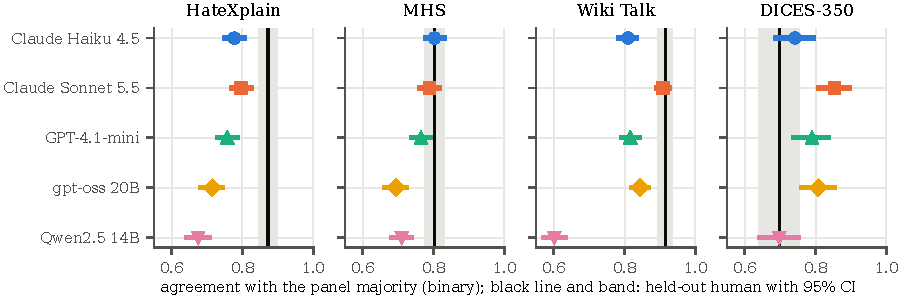
\includegraphics[width=\textwidth]{figures/judges.pdf}
\caption{Judge agreement with the panel majority (95\% bootstrap intervals). The black line and grey band mark a held-out human annotator scored on the same items.}
\label{fig:judges}
\end{figure*}

\begin{table*}[t]
\centering\small
\begin{tabular}{@{}lrrrrrrrr@{}}
\toprule
Judge & \multicolumn{2}{c}{HateXplain} & \multicolumn{2}{c}{MHS} & \multicolumn{2}{c}{Wiki Talk} & \multicolumn{2}{c}{DICES-350} \\
\midrule
Held-out human & 0.872 &  & 0.803 &  & 0.915 &  & 0.697 &  \\
Claude Haiku 4.5 & 0.777 & -0.095 & 0.803 & +0.000 & 0.810 & -0.105 & 0.742 & +0.044 \\
Claude Sonnet 5.5 & 0.796 & -0.077 & 0.788 & -0.015 & 0.908 & -0.006 & 0.853$^{\ast}$ & +0.147 \\
GPT-4.1-mini & 0.757 & -0.115 & 0.765 & -0.038 & 0.816 & -0.099 & 0.790$^{\ast}$ & +0.092 \\
Qwen2.5 14B & 0.675 & -0.198 & 0.710 & -0.093 & 0.601 & -0.314 & 0.697 & +0.000 \\
gpt-oss 20B & 0.715 & -0.158 & 0.694 & -0.109 & 0.844 & -0.071 & 0.808$^{\ast}$ & +0.111 \\
\bottomrule
\end{tabular}

\caption{Agreement with the panel majority and difference from the held-out human (judge $-$ human). $^\ast$Gate~v2 accepts ``judge beats the held-out human'' ($z>2.58$).}
\label{tab:judges}
\end{table*}

\paragraph{On the three toxicity and hate corpora, no judge beats a single human.} The best judge is at or below the held-out human on HateXplain (Sonnet \jSonnetHx vs.\ \jHumanHx), MHS (Haiku \jHaikuMhs vs.\ \jHumanMhs) and Wikipedia Talk (Sonnet \jSonnetWiki vs.\ \jHumanWiki; Table~\ref{tab:judges}, Figure~\ref{fig:judges}). Where the difference is small (Sonnet on Wikipedia Talk, \jDiffSonnetWiki [\jDiffLoSonnetWiki, \jDiffHiSonnetWiki]), the interval includes zero, so the honest statement is ``indistinguishable from one annotator'', not ``human-level''. The weakest judge, Qwen2.5 14B, is \jDiffQwenWiki below the human on Wikipedia Talk.

\paragraph{On DICES, three judges beat an individual rater, and this says more about the rater than the judges.} DICES has $\alpha\approx$ \alphaDthree, so a single rater is a weak reference: the held-out human reaches only \jHumanDthree. Sonnet (\jSonnetDthree), gpt-oss (\jOssDthree) and GPT-4.1-mini (\jGptDthree) exceed it, and gate~v2 accepts each claim. Against the dataset's expert safety labels, however, every judge (\jExpertQwen--\jExpertSonnet) is close to or below the held-out crowd rater (\jExpertHuman) and below the crowd panel's majority (\jExpertPanel). Beating a noisy individual is not the same as measuring the construct better.

\paragraph{The Sonnet result on DICES is fragile.} On \jSonnetDthreeUnparsed of 350 DICES conversations, Sonnet began explaining and reached its output limit before giving a label; no model refused any item (\jRefusals refusals in total), and no other judge--corpus pair had more than \jOtherInvalidMax unusable outputs. The pre-registered analysis excludes such outputs; scored as wrong, Sonnet's agreement falls from \jSonnetDthree to \jSonnetDthreeInvalidWrong, barely above the human. We did not re-run with a larger limit, because that would be a post-hoc change to a measured judge.

\paragraph{Alternative Annotator Test.} With the paper's default for crowd annotators ($\varepsilon=0.1$, Benjamini--Yekutieli at $q=0.05$), the test applies to HateXplain (\altAnnotHx annotators with at least 30 items) and DICES (\altAnnotDthree), and to neither MHS nor Wikipedia Talk, where no annotator has 30 items in the sample. No judge passes on HateXplain (winning rates \altQwenHx--\altHaikuHx, against the 0.5 required). On DICES four judges pass, Sonnet with a winning rate of \altSonnetDthree, consistent with the DICES result above. The test's requirement of dense annotation is itself a practical limit: most benchmarks cannot run it.

\paragraph{Comparing judges.} Gate~v2 resolves the direction of \jPairsPass of the \jPairsTotal judge-versus-judge comparisons; all \jPairsClose comparisons with gaps under 0.02 stay unresolved (\jPairsClosePass pass). A leaderboard of these judges built from the same samples could order the extremes but not the neighbours.
